\textit{Примечание:} везде, если не оговорено иное, имеются в виду правые и левые берега рек \textbf{орографически}.

\textbf{Отчёт писали:} Даша Снеговская, Лёша Остапив, Даша Казаринова, Вика Суровцева, Дима Дёмушкин, Катя Тюрина, Илья Шалфеев, Дима Сингалевич.
\subsection{18 августа. Старт}
\textit{Метеоусловия: утром, днём, вечером ясно, тепло.}

\begin{figure}[h!]
	\centering
	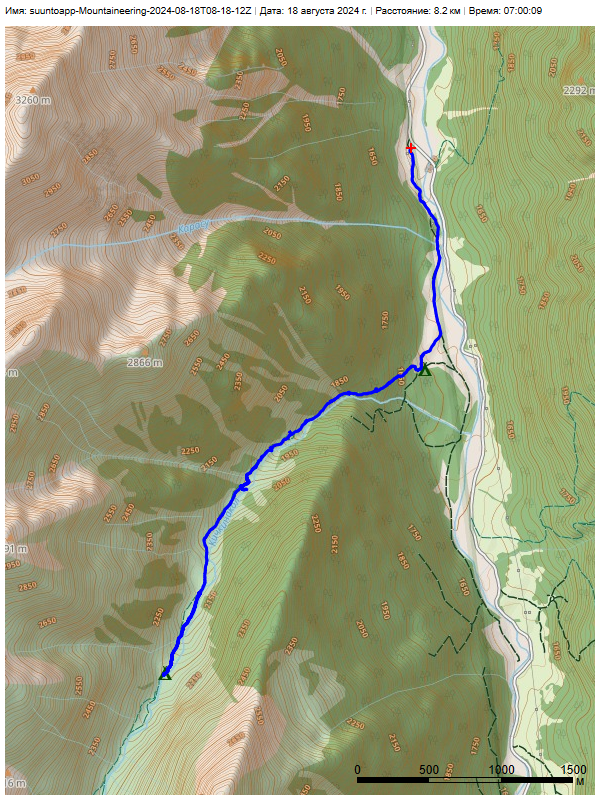
\includegraphics[angle=0, width=0.7\linewidth]{../pics/mini_maps/18}
	\label{fig:mini_18}
\end{figure}

Прибыли в г. Минеральные Воды в 03:40. Встретились на вокзале с участником, прибывшим на день раньше, и загрузились в машину Бориса Саракуева. В 04:00 отправились на место старта (мост через р. Учкулан, N 43.38668\degree~E 41.98961\degree), куда прибыли в 09:45 (По дороге на 40 минут остановились в ауле Учкулан, чтобы позавтракать). Распределили заброски, отдали их водителю и выдвинулись на маршрут в 11:18. Первые 1.5 км до коша шли по д.р. Учкулан, затем тропа повела через калитку и повернула направо, на подъём в висячую долину р. Кичкинакол Джалпаккольский.

\begin{figure}[h!]
	\centering
	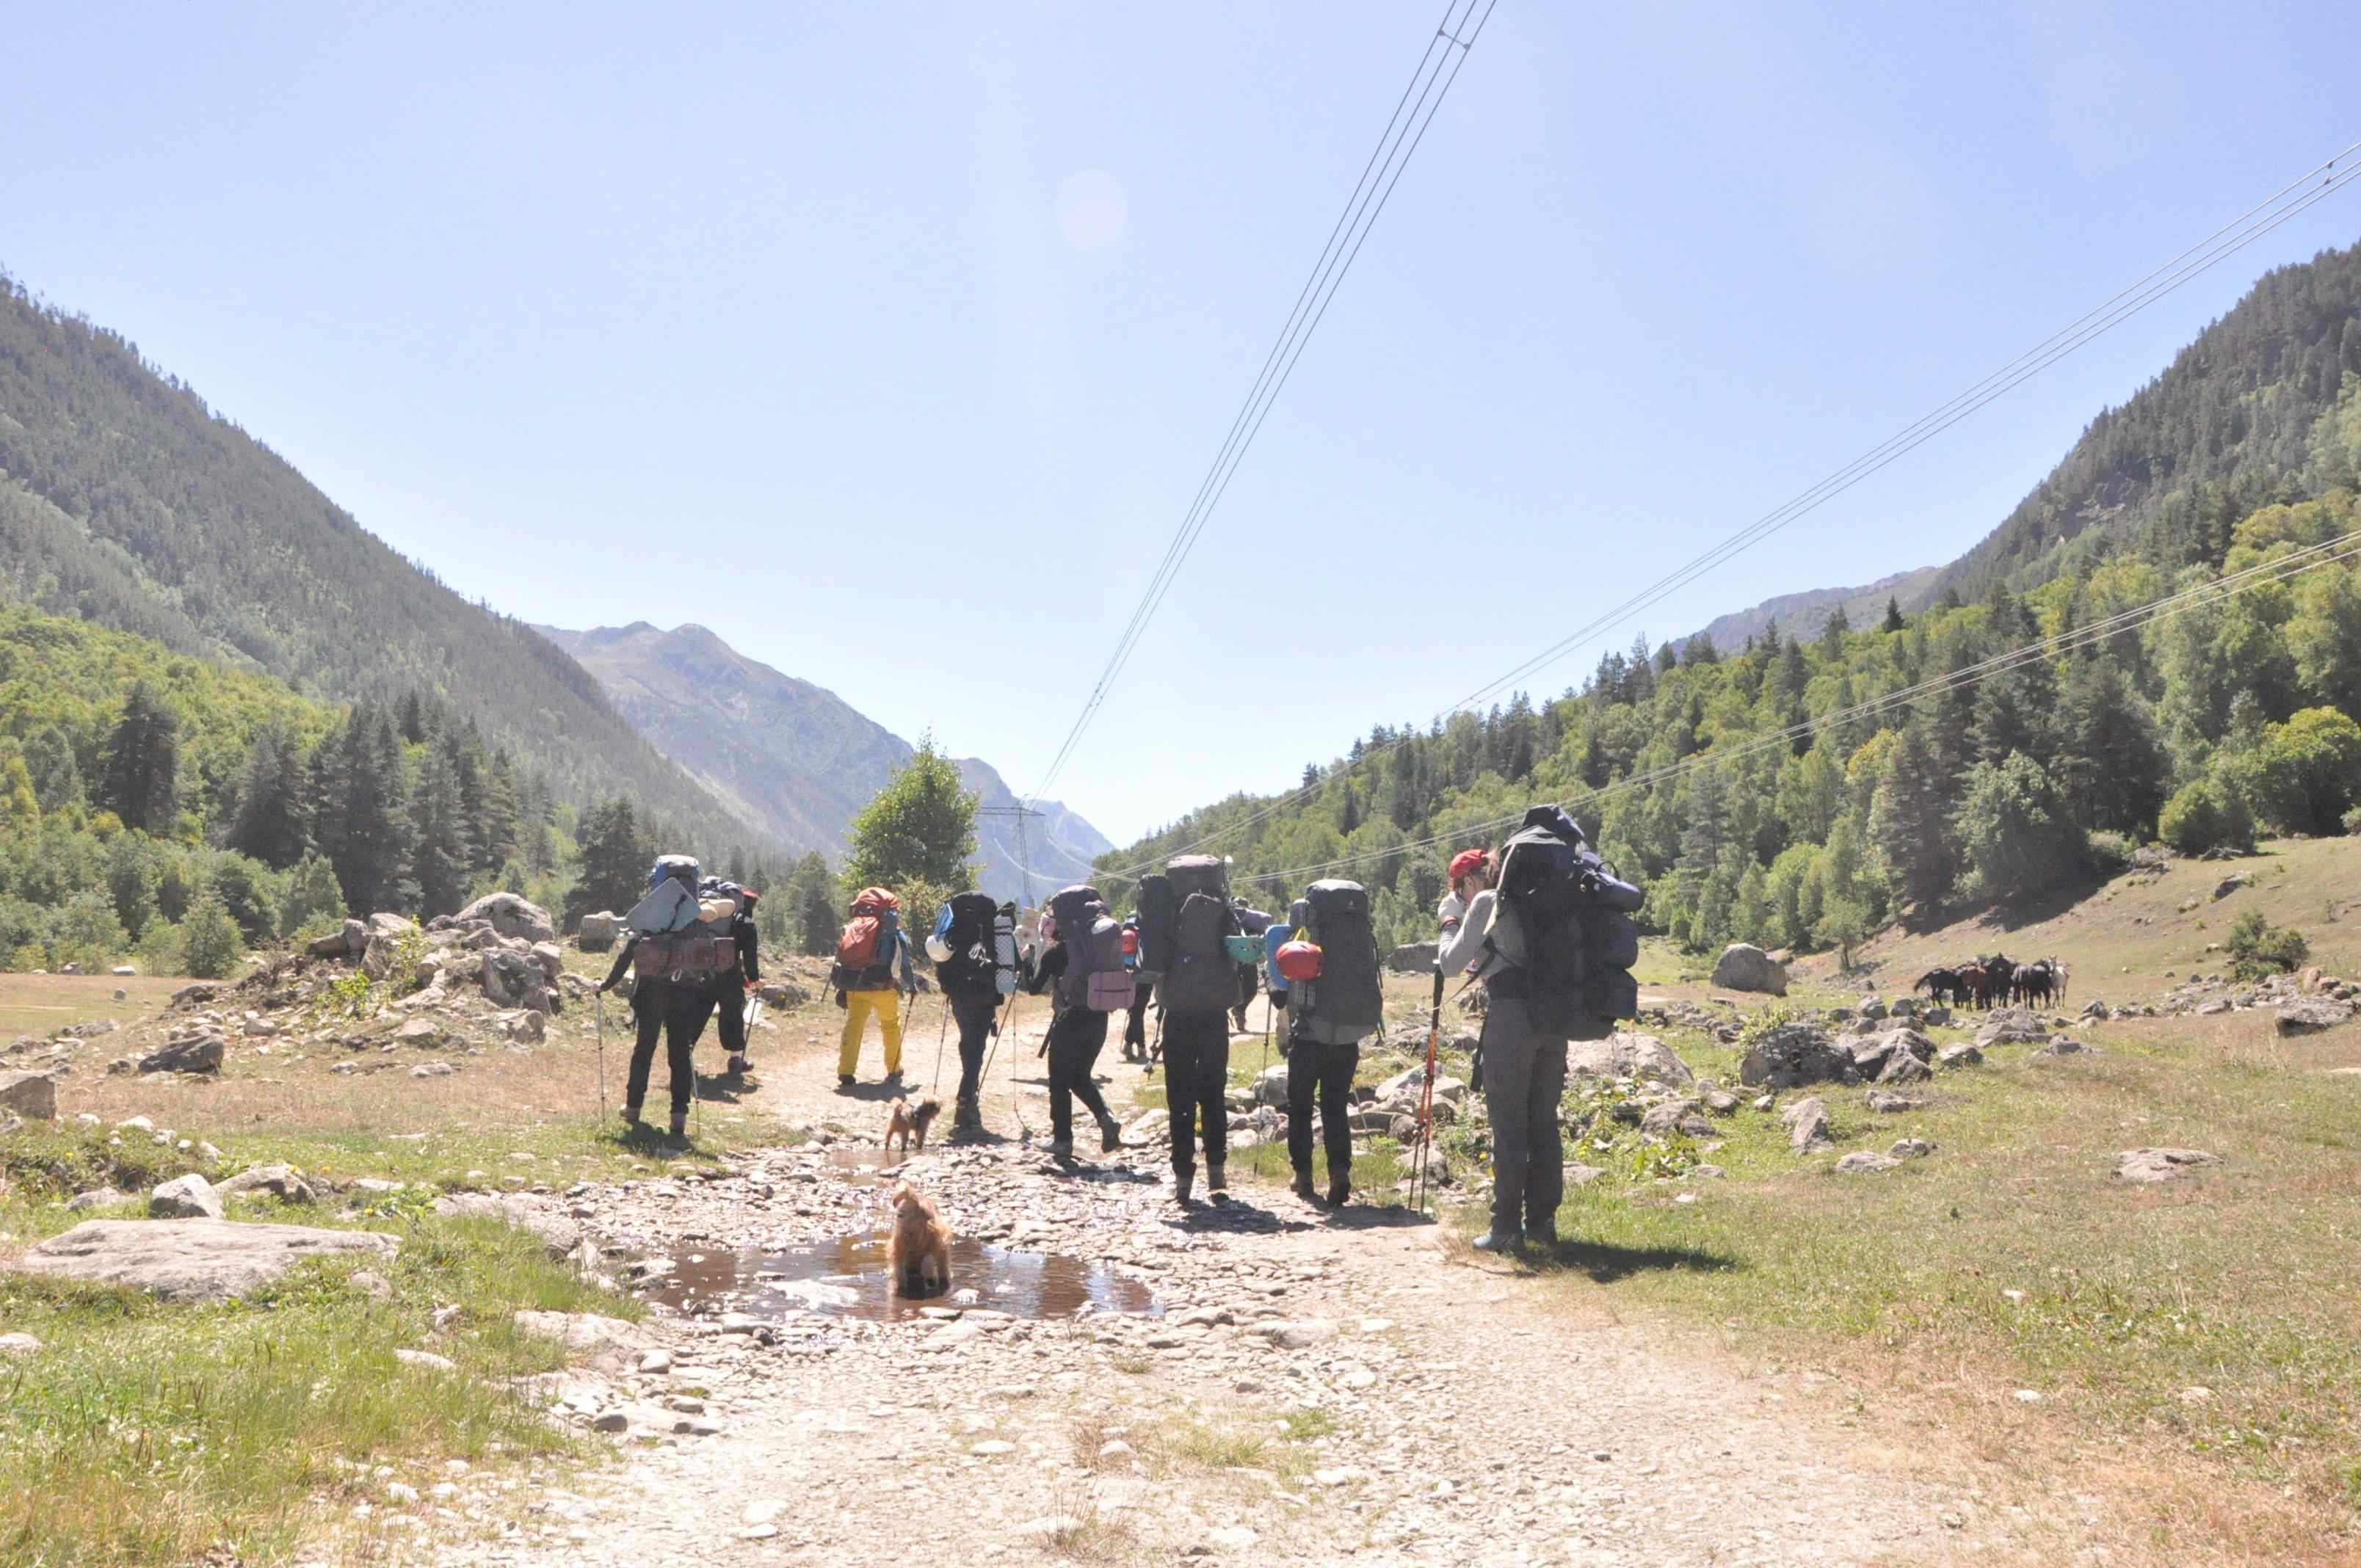
\includegraphics[width=0.7\linewidth]{../pics/DSC_0412}
	\caption{группа на старте маршрута в д.р. Учкулан}
	\label{fig:uchkulan}
\end{figure}

\begin{figure}[h!]
	\centering
	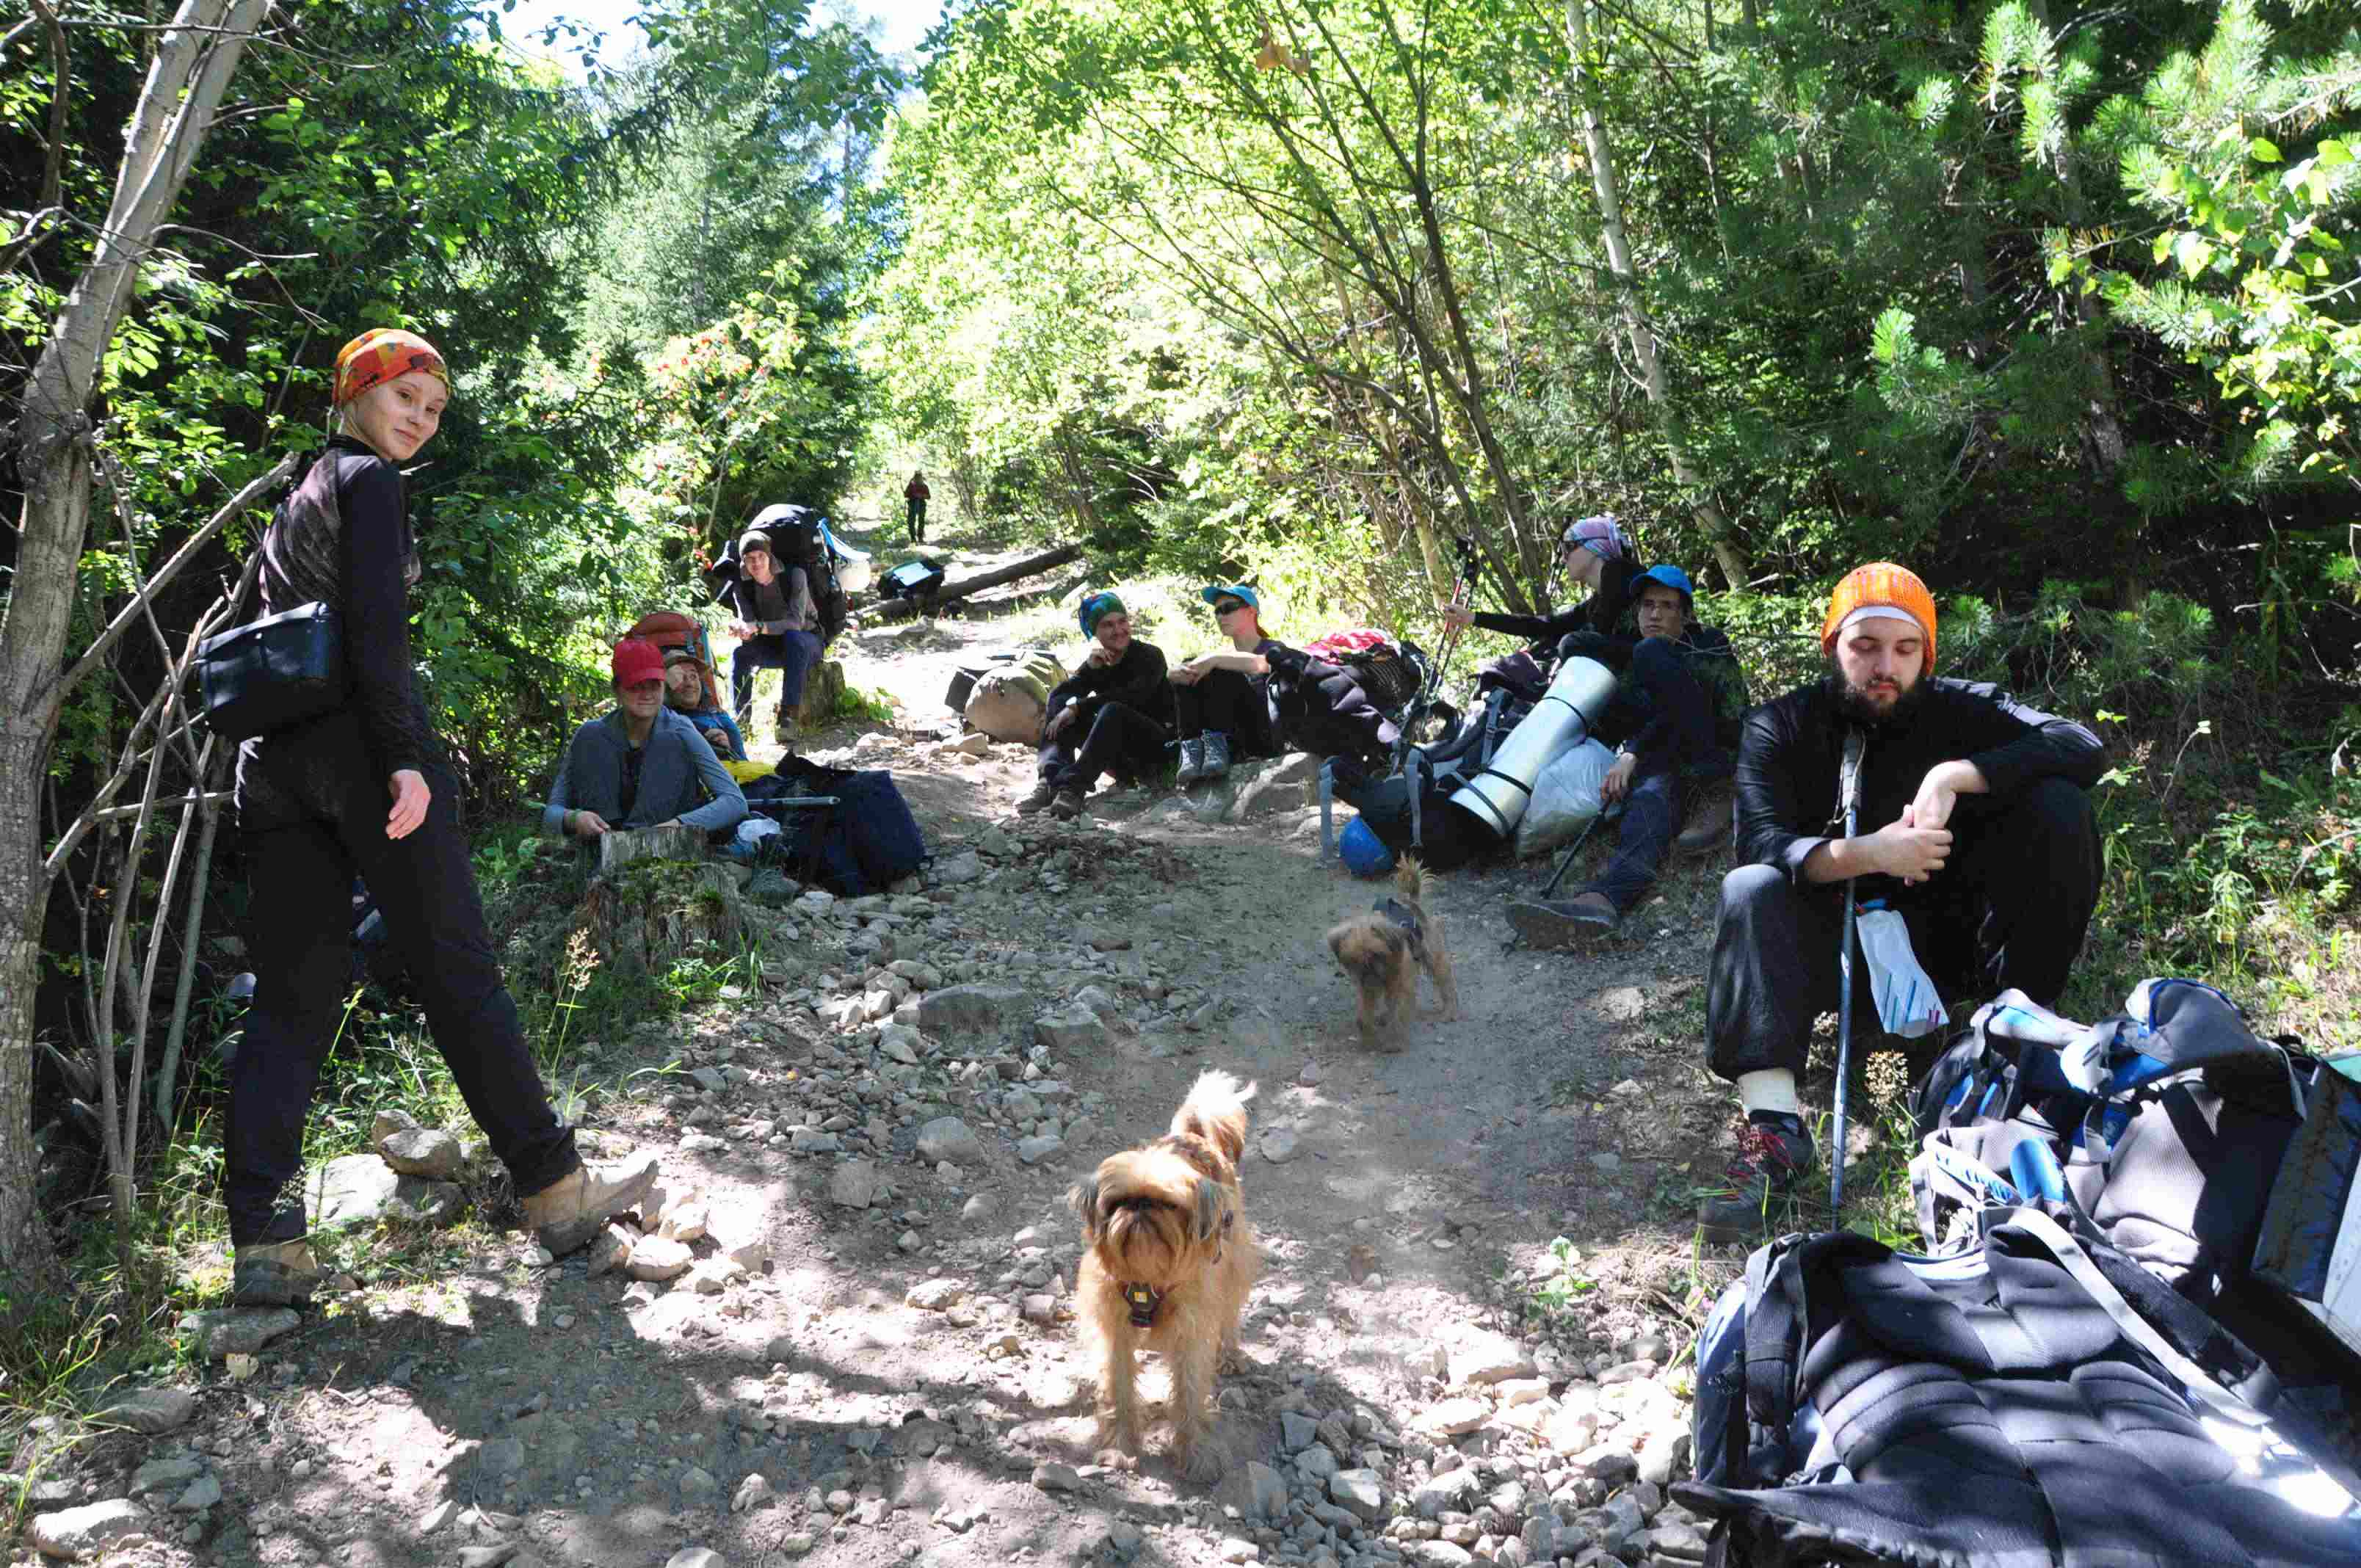
\includegraphics[width=0.7\linewidth]{../pics/DSC_0436}
	\caption{Подъём по тропе в д.р. Кичкинакол Уллукёльский}
	\label{fig:DSC_0436}
\end{figure}

Подъём здесь идёт по хорошей тропе со средним уклоном порядка 20\degree (рис.~\ref{fig:DSC_0436}). Шли не спеша, в режиме 20/5 и далее вплоть до 10/10, разгружая отстающих участников. В 14:30 завершили подъём в долину и устроили обед.

\begin{figure}[h!]
	\centering
	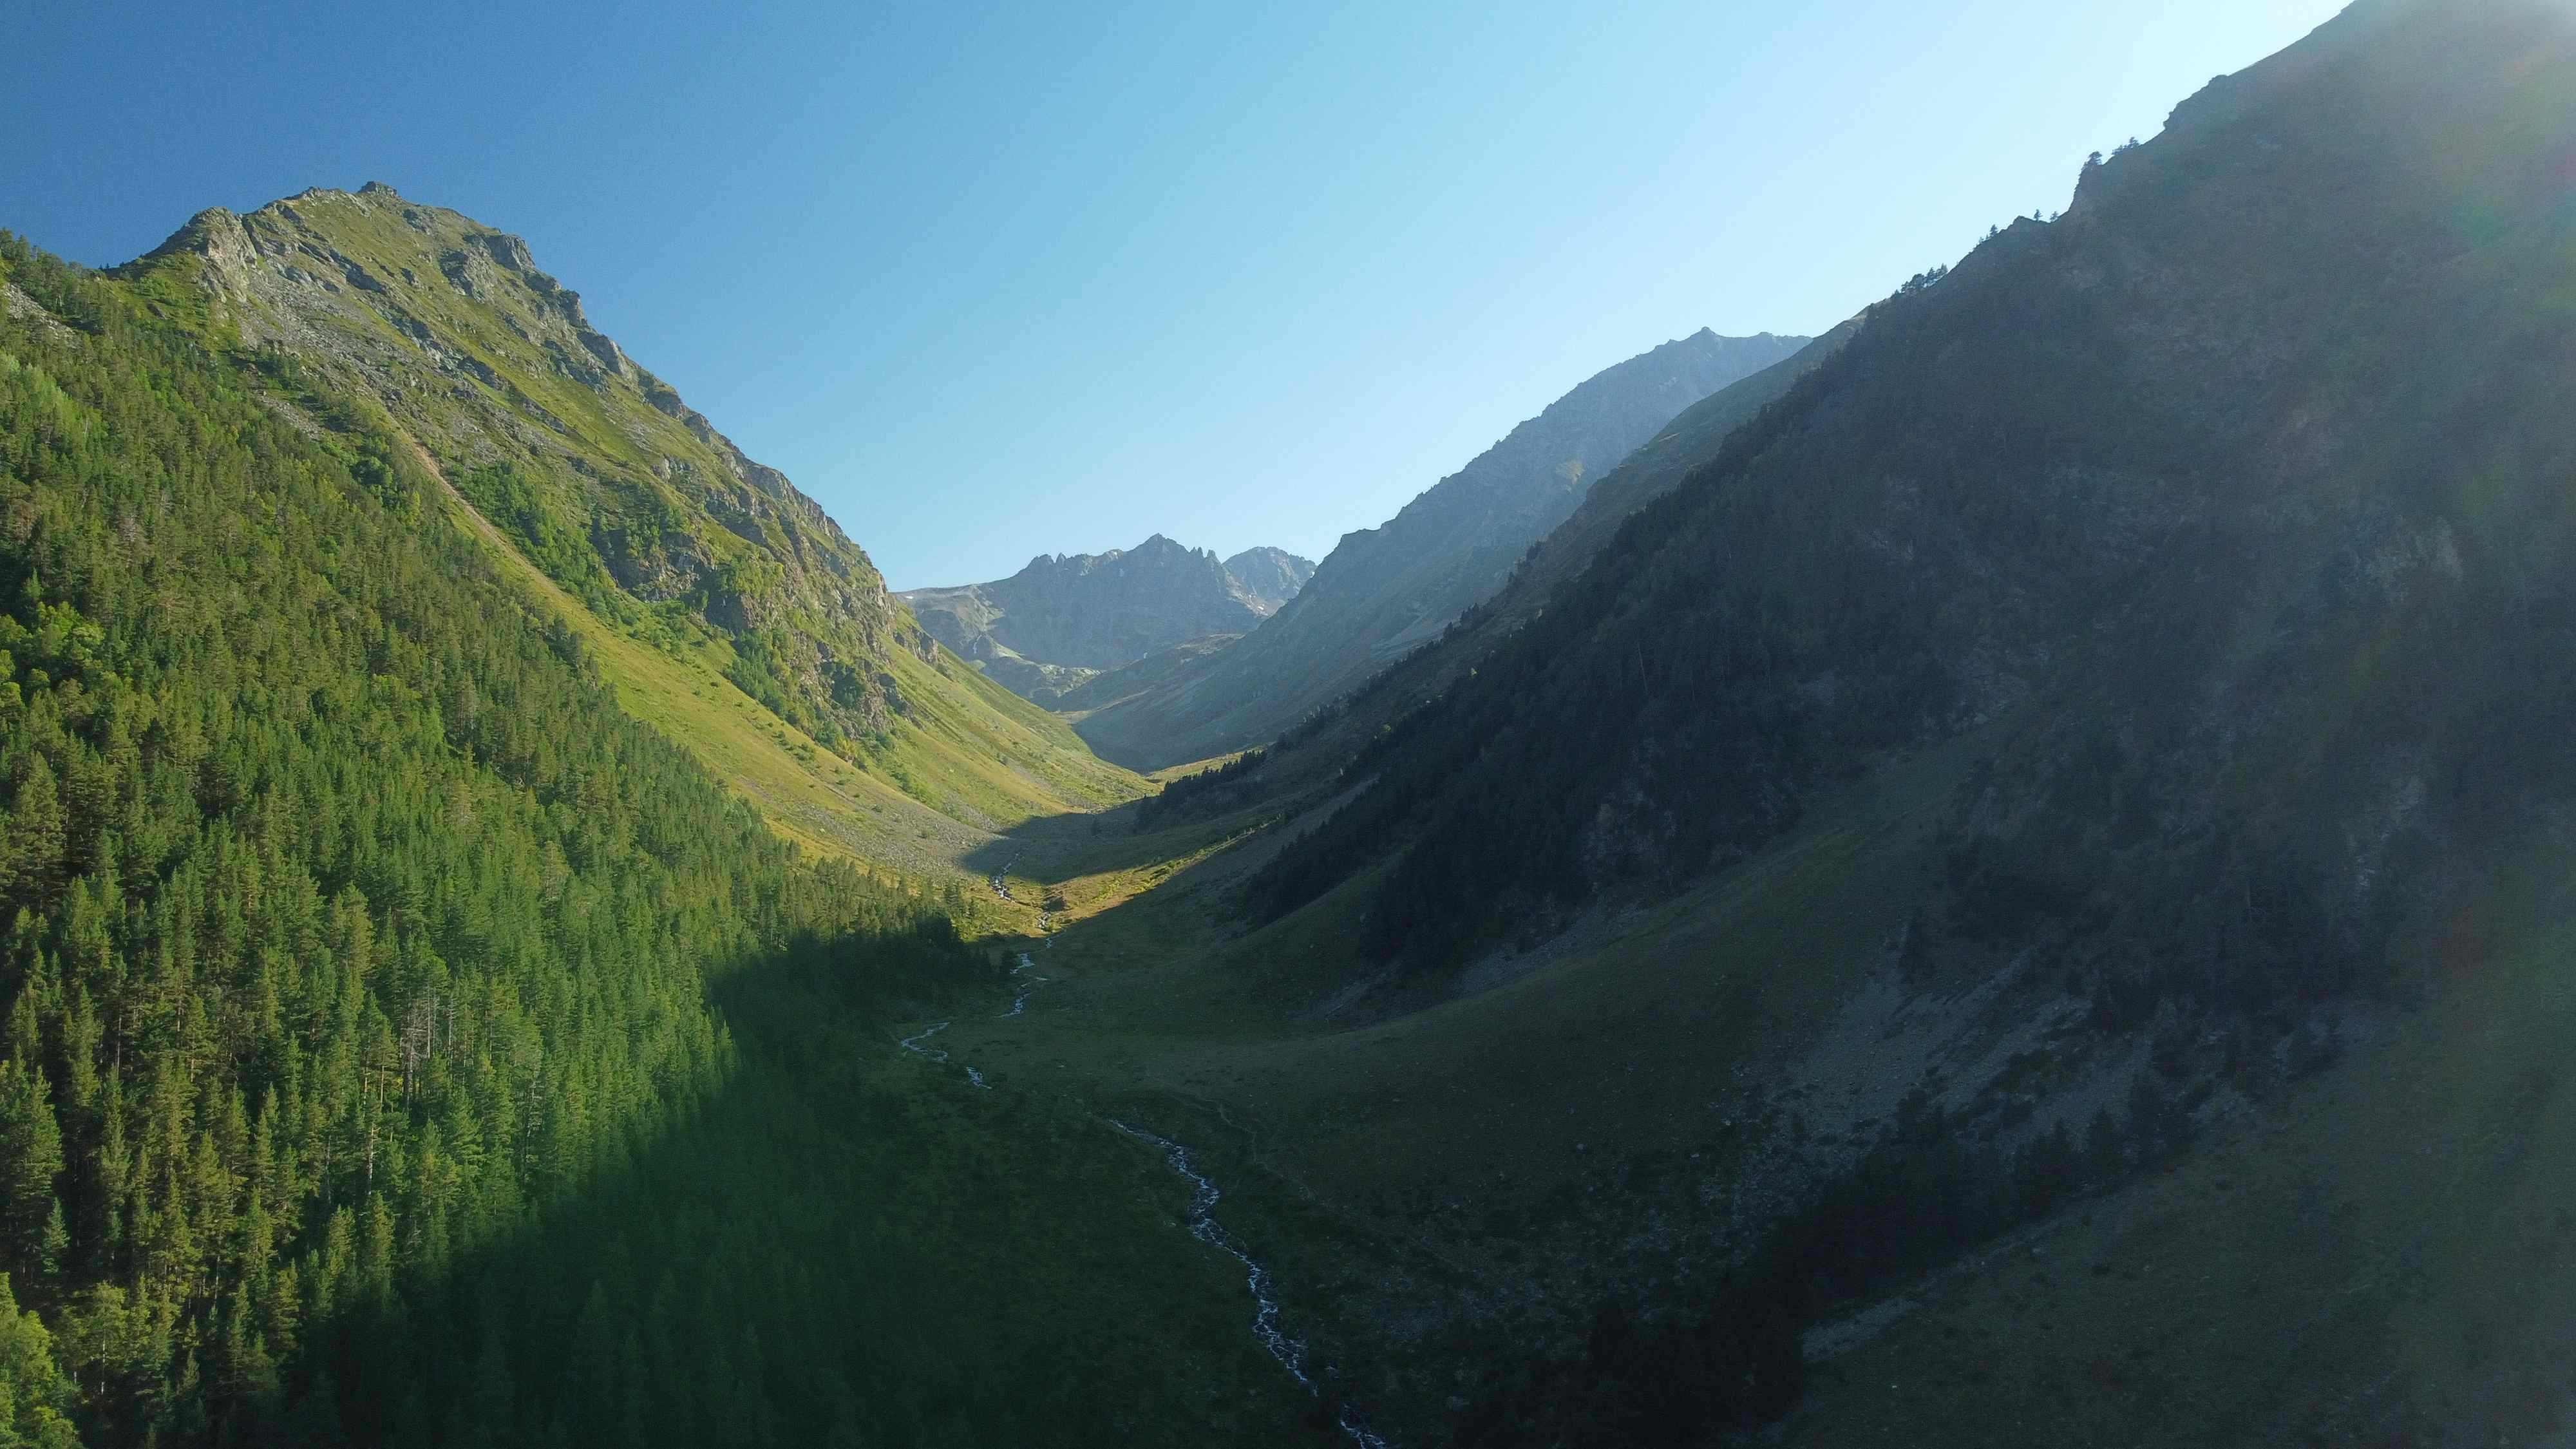
\includegraphics[width=0.7\linewidth]{../pics/DJI_0805}
	\caption{д.р. Кичкинакол Джалпаккольский}
	\label{fig:kichkinakol}
\end{figure}

С обедом закончили в 16:40 и прошли 2 км к оборудованной стоянке возле коша, где оказались в 17:25. Рядом местные жители собирали малину. Подумав немного и устроив разведку, поднялись ещё немного выше и в 18:18 встали на место ночёвки на оборудованной стоянке возле дерева на небольшом разливе реки. Координаты м.н. N 43.35392\degree~E 41.96858\degree.
\begin{figure}[h!]
	\centering
	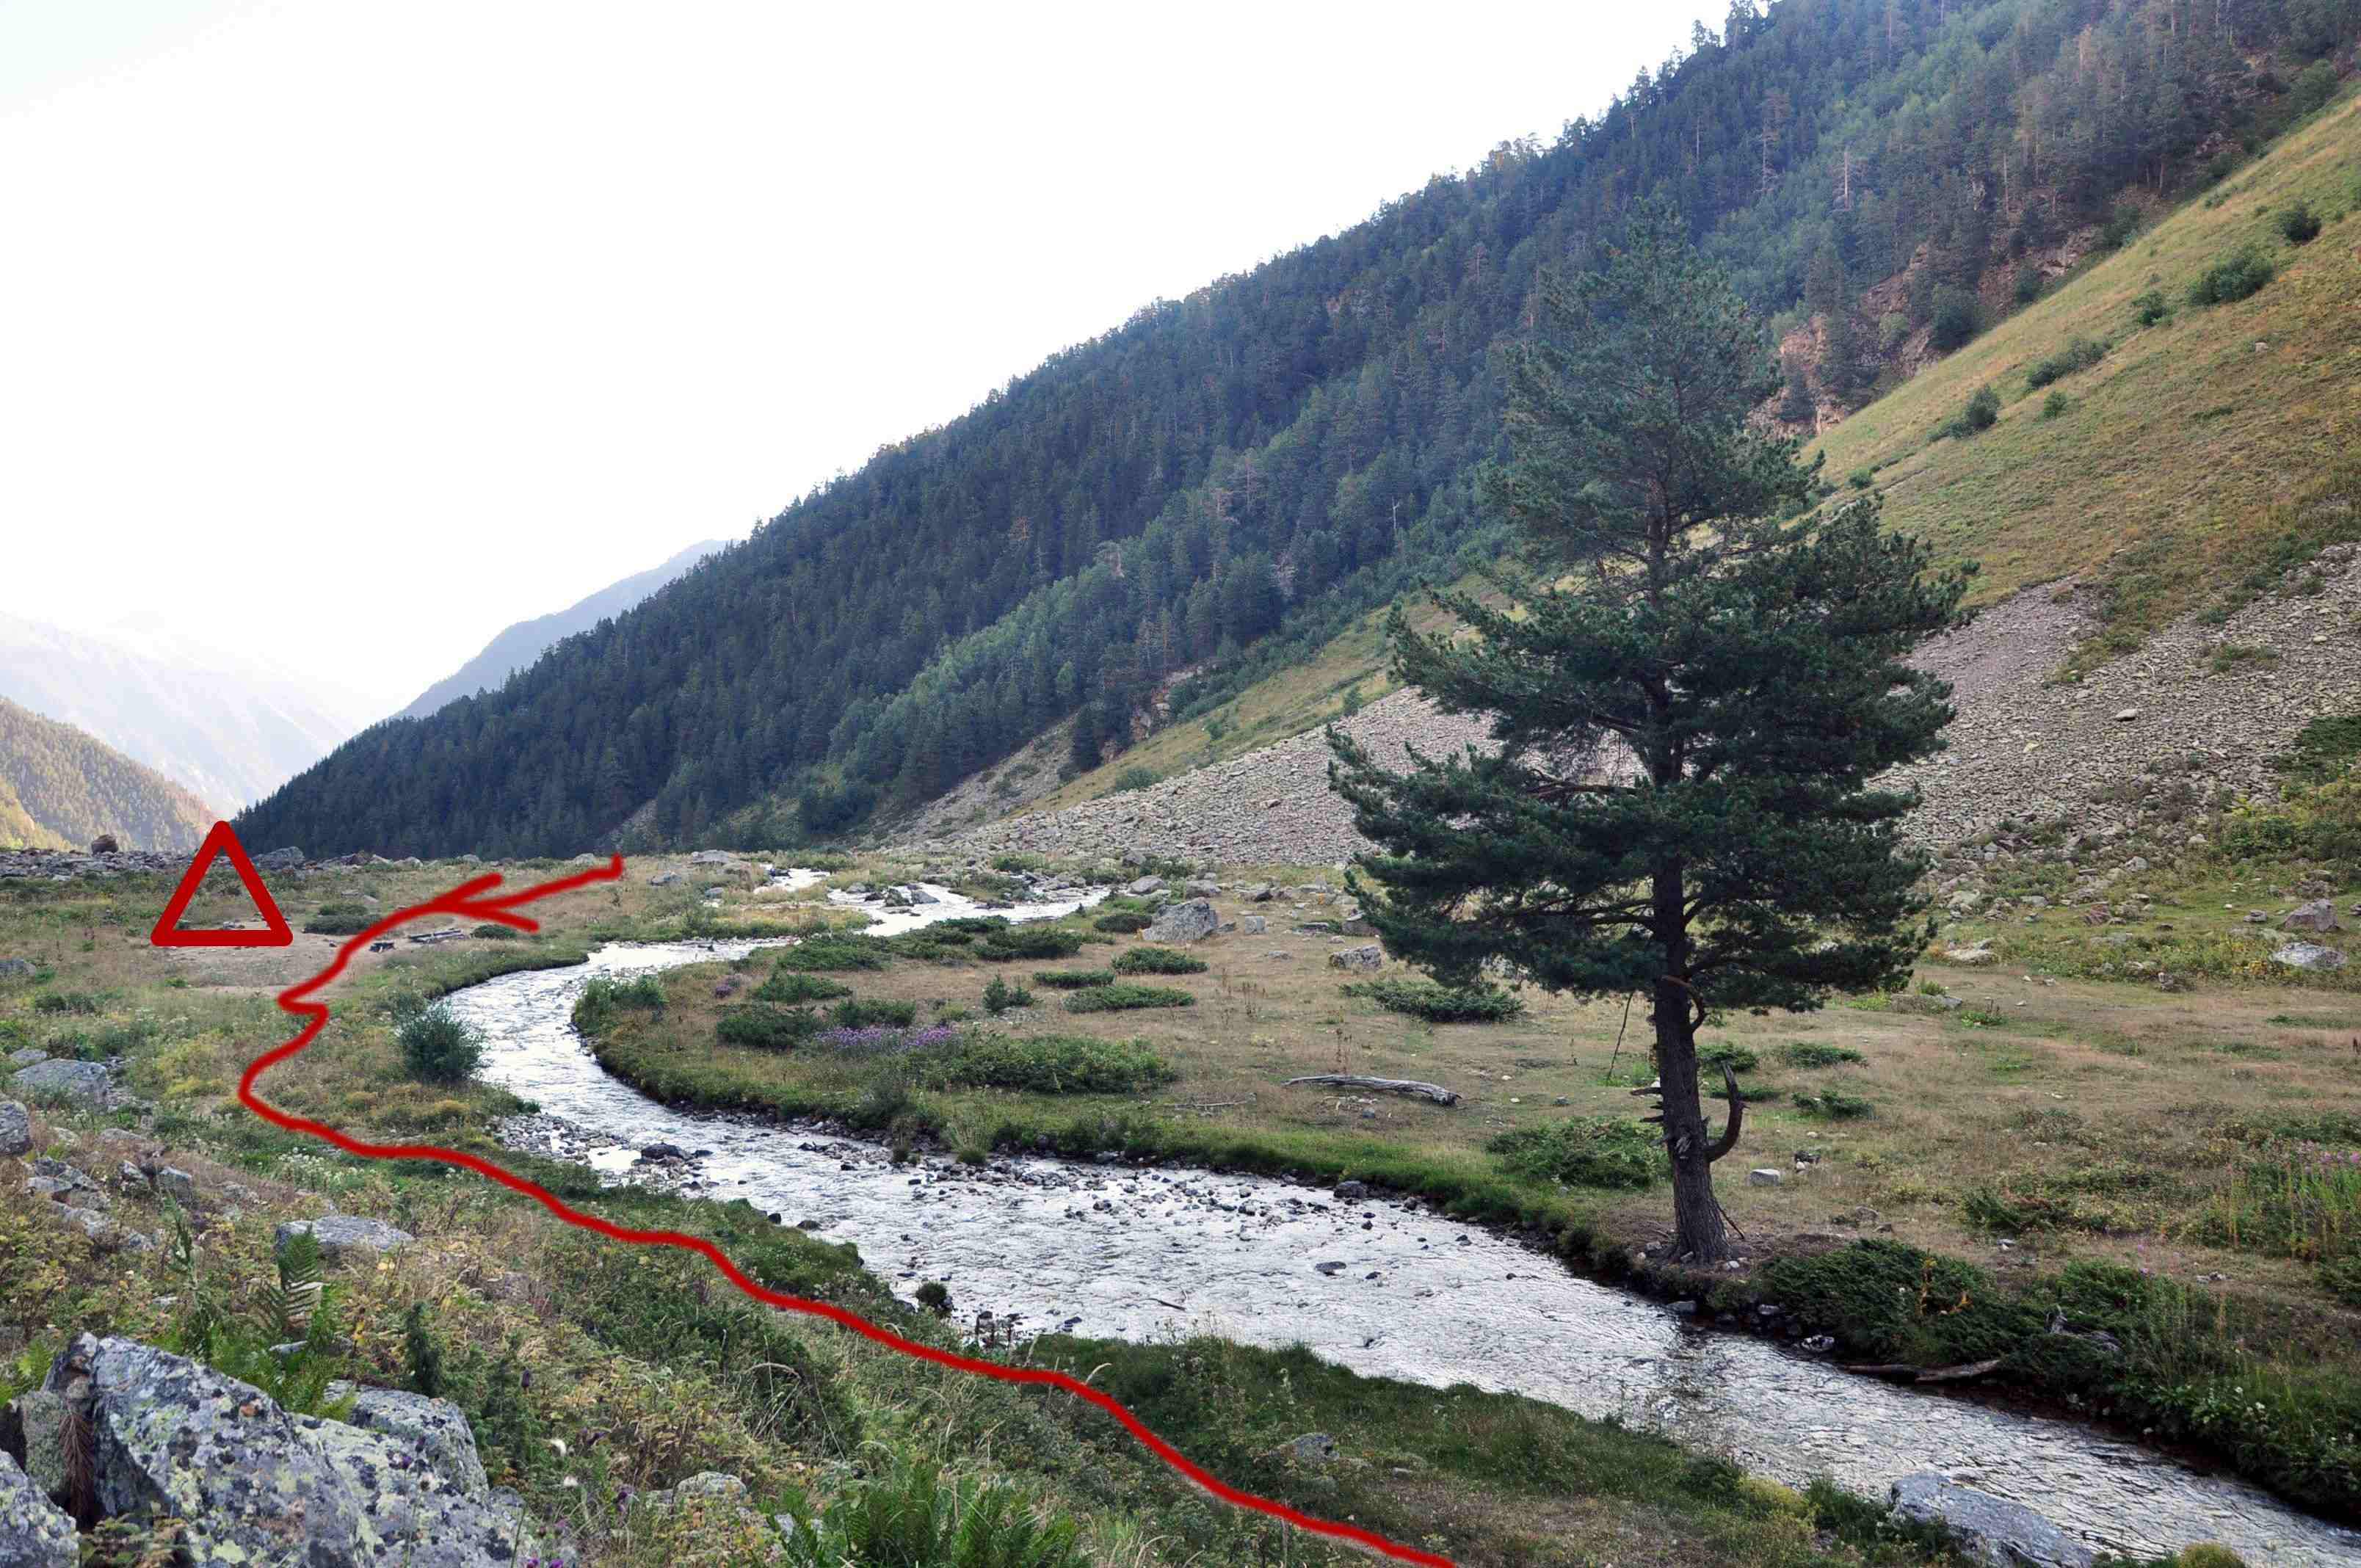
\includegraphics[width=0.7\linewidth]{../pics/camp_18}
	\caption{Место ночёвки 18-19.08}
	\label{fig:camp_18}
\end{figure}

\clearpage